\chapter{Barplots of the average approach} \label{ch: appendix average approach}

The barplots illustrated here stem from an \onehot{} model using a german book to collect the training data. It achieved the best value ($ 7.3 \cdot 10^{-2} $) of the four tested models. The scores are listed in \tabref{\ref{tab: avg model versions and metrics}}. If a \postag{} doesn't appear in the plots \ie having no green or blue bar, this means that it doesn't succeed the depicted \postag{}. The explanation of the \postag{s} can be found in \tabref{\ref{tab: ud pos tags}}.
\begin{figure}[H]
	\centering
		\subcaptionbox{Averaged transitions of all \texttt{ADP}s compared to the ground truth.}{
			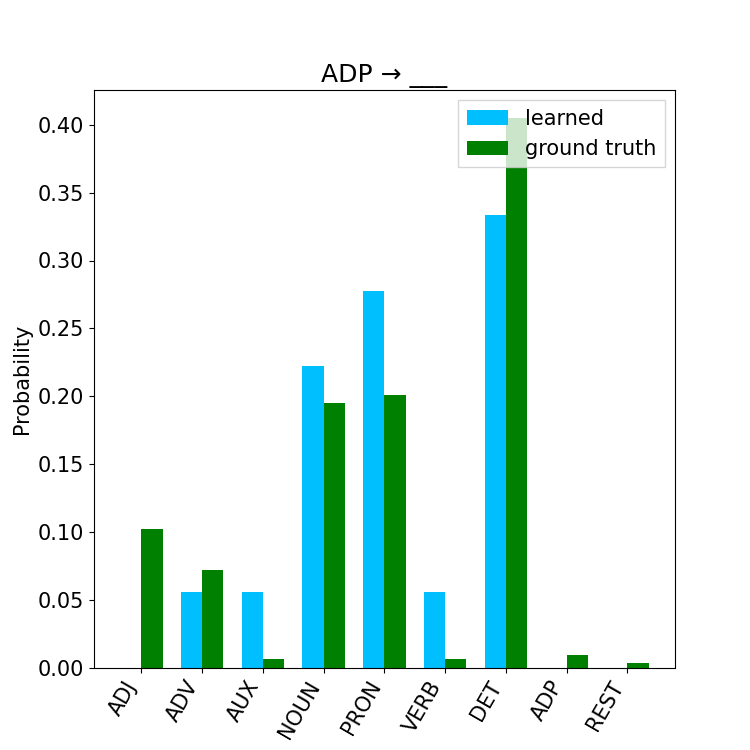
\includegraphics[width=\twocolpicwidth]{Bilder/chapter4/Barplots/Avg_OHE_OHE_5000E_100BS_1L_1C_200P_1500T_D/_epoch-4000/Combined_Barplot_ADP_S.png}
		}
		\hfill
		\subcaptionbox{Averaged transitions of all \texttt{ADJ}s compared to the ground truth.}{
			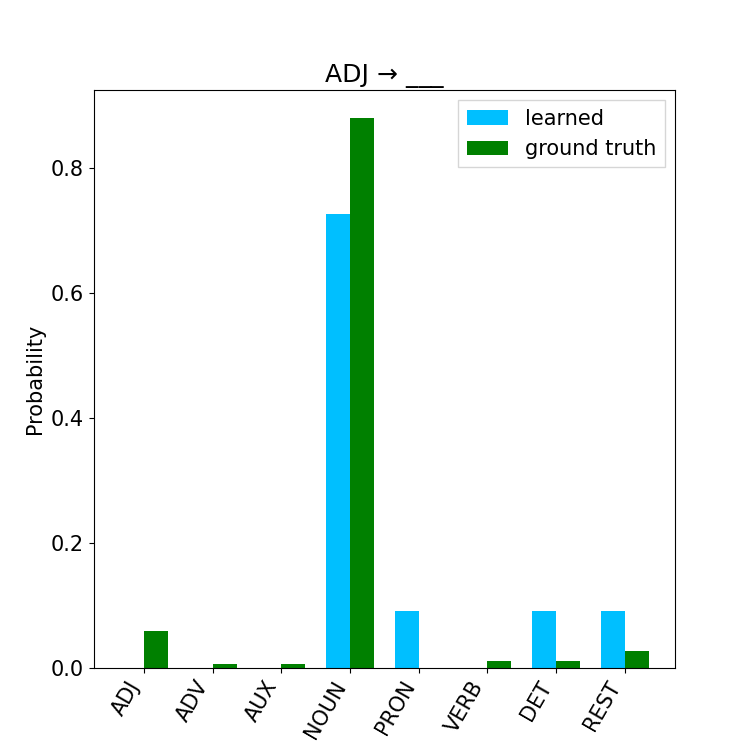
\includegraphics[width=\twocolpicwidth]{Bilder/chapter4/Barplots/Avg_OHE_OHE_5000E_100BS_1L_1C_200P_1500T_D/_epoch-4000/Combined_Barplot_ADJ_F.png}
		}
	\caption{Barplot of \texttt{ADP} and \texttt{ADJ}.}
\end{figure}
\begin{figure}[H]
	\centering
	\subcaptionbox{Averaged transitions of all \texttt{DET}s compared to the ground truth.}{
		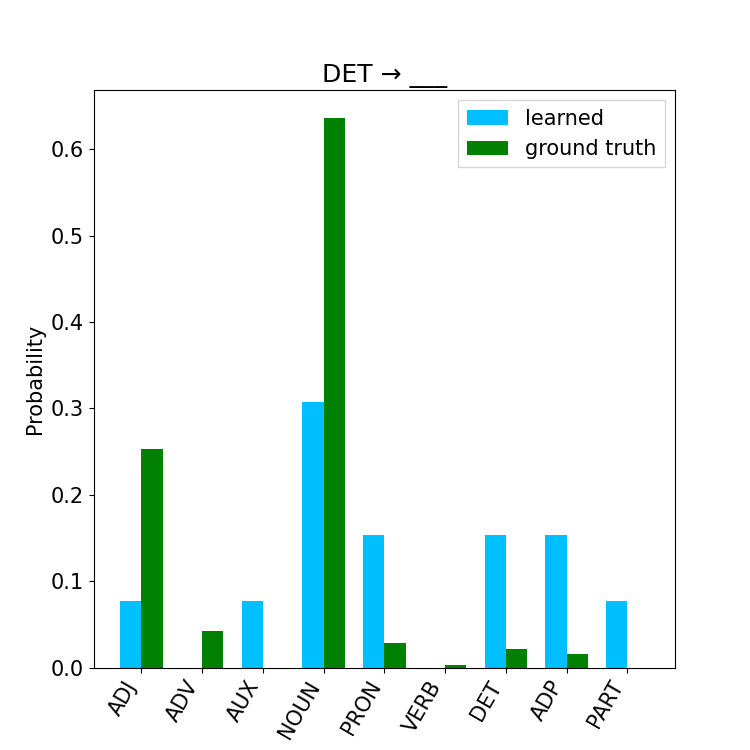
\includegraphics[width=\twocolpicwidth]{Bilder/chapter4/Barplots/Avg_OHE_OHE_5000E_100BS_1L_1C_200P_1500T_D/_epoch-4000/Combined_Barplot_DET_S.png}
	}
	\hfill
	\subcaptionbox{Averaged transitions of all \texttt{ADV}s compared to the ground truth.}{
		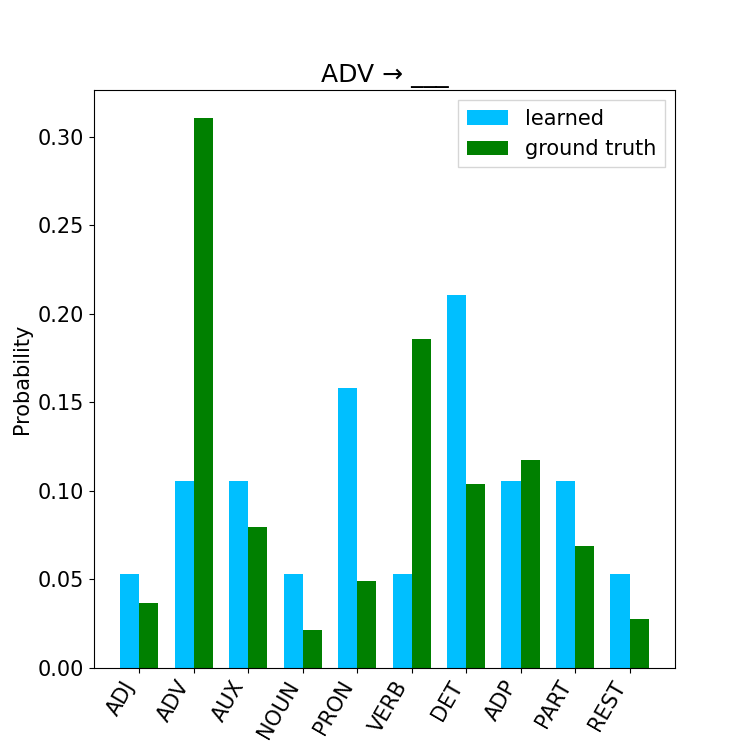
\includegraphics[width=\twocolpicwidth]{Bilder/chapter4/Barplots/Avg_OHE_OHE_5000E_100BS_1L_1C_200P_1500T_D/_epoch-4000/Combined_Barplot_ADV_F.png}
	}
	\caption{Barplot of \texttt{DET} and \texttt{ADV}.}
\end{figure}
\begin{figure}[H]
	\centering
	\subcaptionbox{Averaged transitions of all \texttt{AUX}s compared to the ground truth.}{
		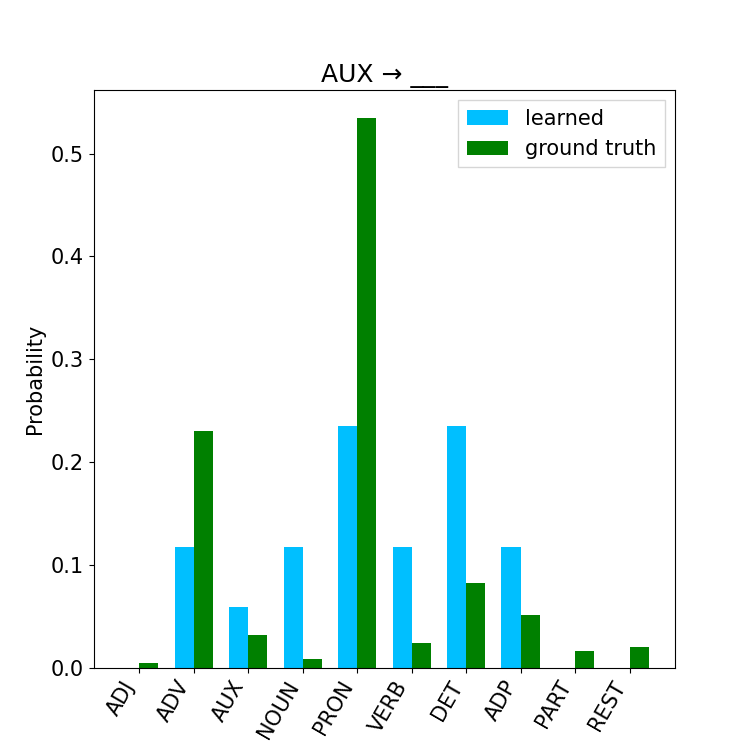
\includegraphics[width=\twocolpicwidth]{Bilder/chapter4/Barplots/Avg_OHE_OHE_5000E_100BS_1L_1C_200P_1500T_D/_epoch-4000/Combined_Barplot_AUX_F.png}
	}
	\hfill
	\subcaptionbox{Averaged transitions of all \texttt{NOUN}s compared to the ground truth.}{
		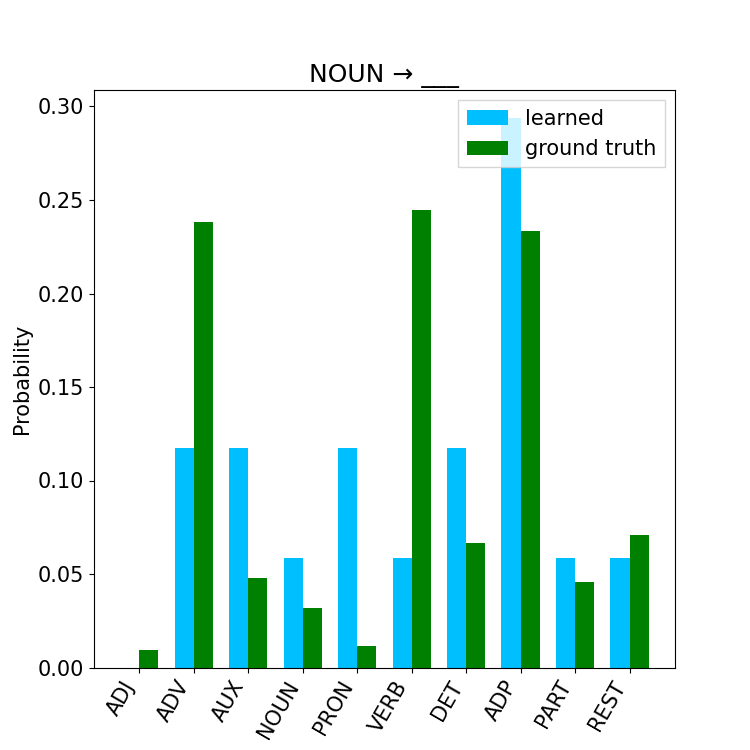
\includegraphics[width=\twocolpicwidth]{Bilder/chapter4/Barplots/Avg_OHE_OHE_5000E_100BS_1L_1C_200P_1500T_D/_epoch-4000/Combined_Barplot_NOUN_F.png}
	}
	\caption{Barplot of \texttt{AUX} and \texttt{NOUN}.}
\end{figure}
\begin{figure}[H]
	\centering
	\subcaptionbox{Averaged transitions of all \texttt{VERB}s compared to the ground truth.}{
		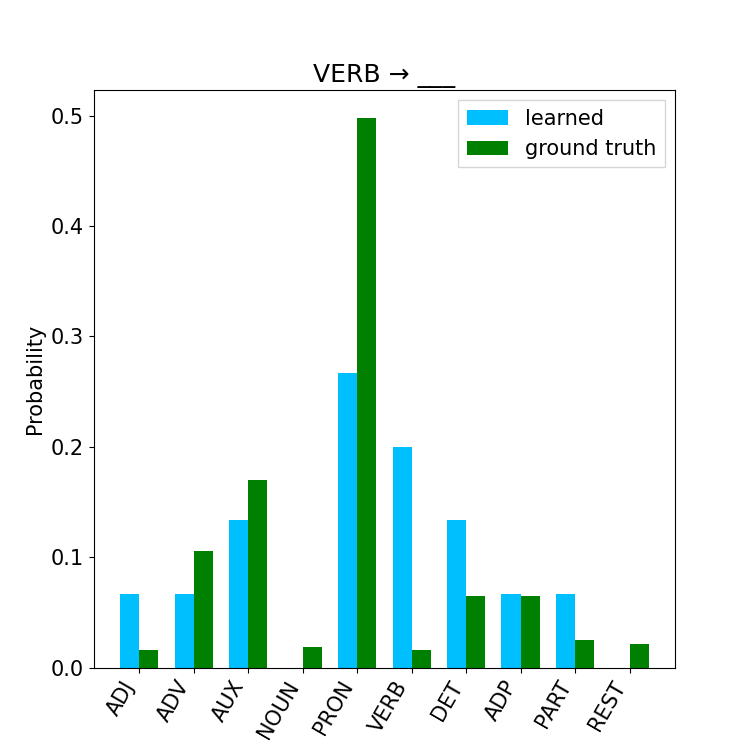
\includegraphics[width=\twocolpicwidth]{Bilder/chapter4/Barplots/Avg_OHE_OHE_5000E_100BS_1L_1C_200P_1500T_D/_epoch-4000/Combined_Barplot_VERB_S.png}
	}
	\hfill
	\subcaptionbox{Averaged transitions of all \texttt{REST}s compared to the ground truth.}{
		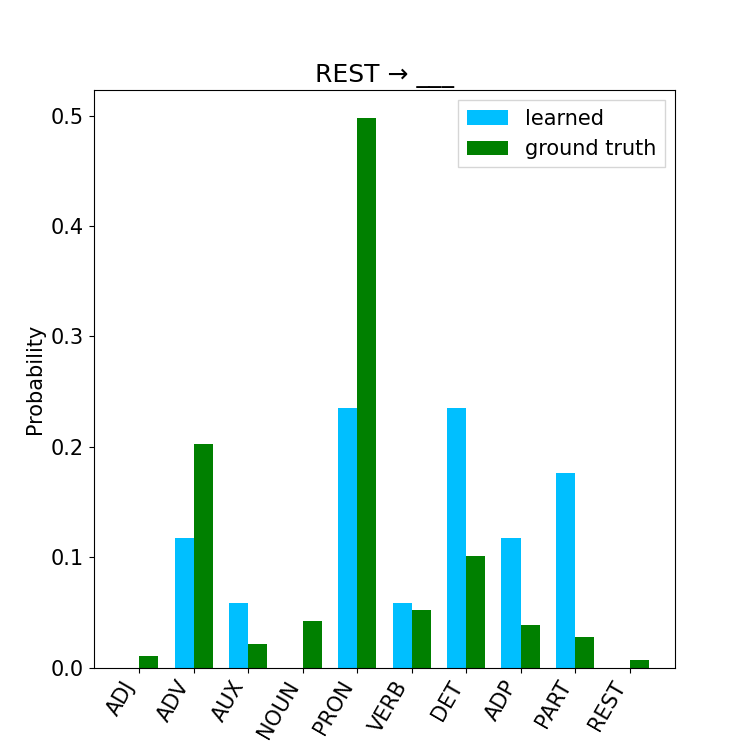
\includegraphics[width=\twocolpicwidth]{Bilder/chapter4/Barplots/Avg_OHE_OHE_5000E_100BS_1L_1C_200P_1500T_D/_epoch-4000/Combined_Barplot_REST_S.png}
	}
	\caption{Barplot of \texttt{VERB} and \texttt{REST}.}
\end{figure}
\begin{figure}[H]
	\centering
	\subcaptionbox{Averaged transitions of all \texttt{PART}s compared to the ground truth.}{
		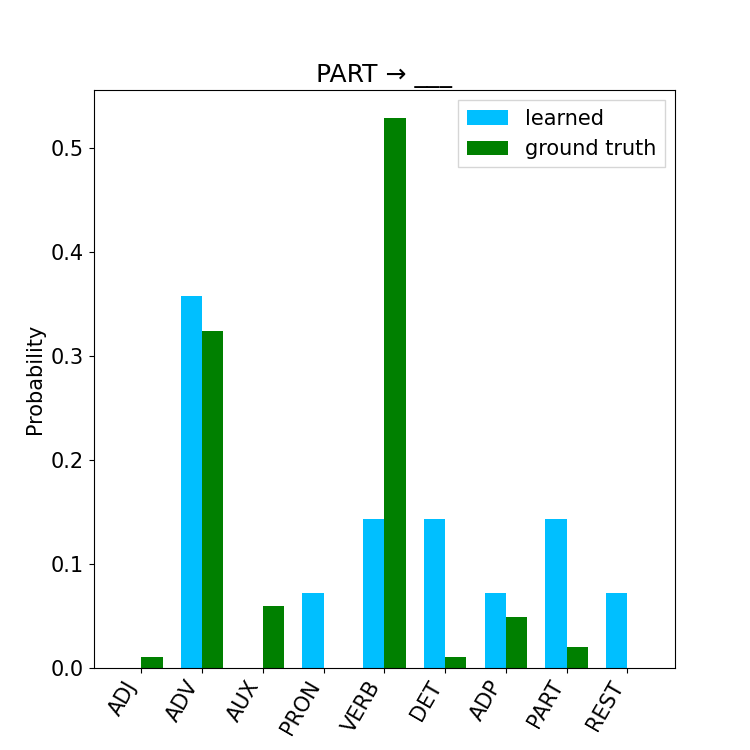
\includegraphics[width=\twocolpicwidth]{Bilder/chapter4/Barplots/Avg_OHE_OHE_5000E_100BS_1L_1C_200P_1500T_D/_epoch-4000/Combined_Barplot_PART_S.png}
	}
	\hfill
	\subcaptionbox{Averaged transitions of all \texttt{PRON}s compared to the ground truth.}{
		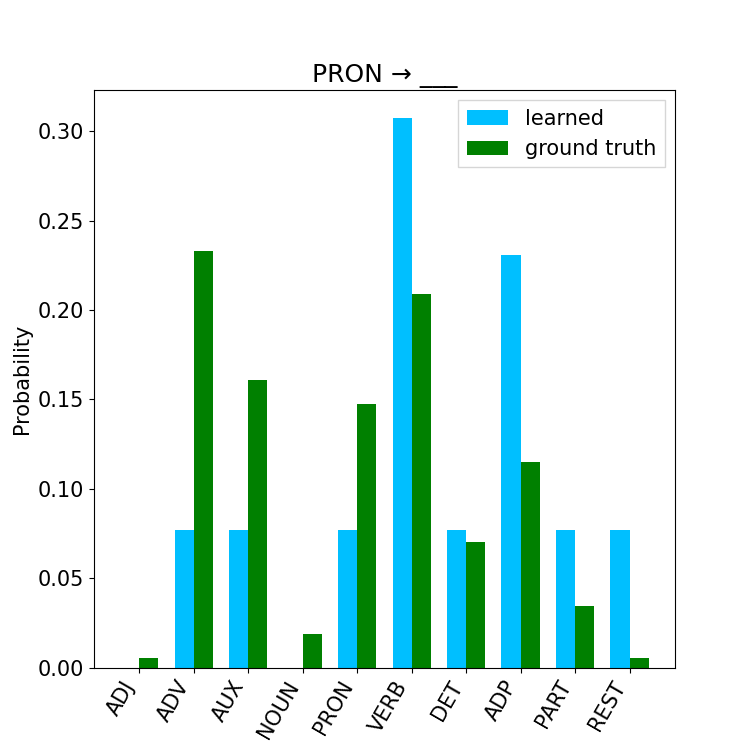
\includegraphics[width=\twocolpicwidth]{Bilder/chapter4/Barplots/Avg_OHE_OHE_5000E_100BS_1L_1C_200P_1500T_D/_epoch-4000/Combined_Barplot_PRON_F.png}
	}
	\caption{Barplot of \texttt{PART} and \texttt{PRON}.}
\end{figure}
